\subsection*{ГЛ14 4}
\begin{enumerate}
\item[(а)]
	\begin{figure}[h]
		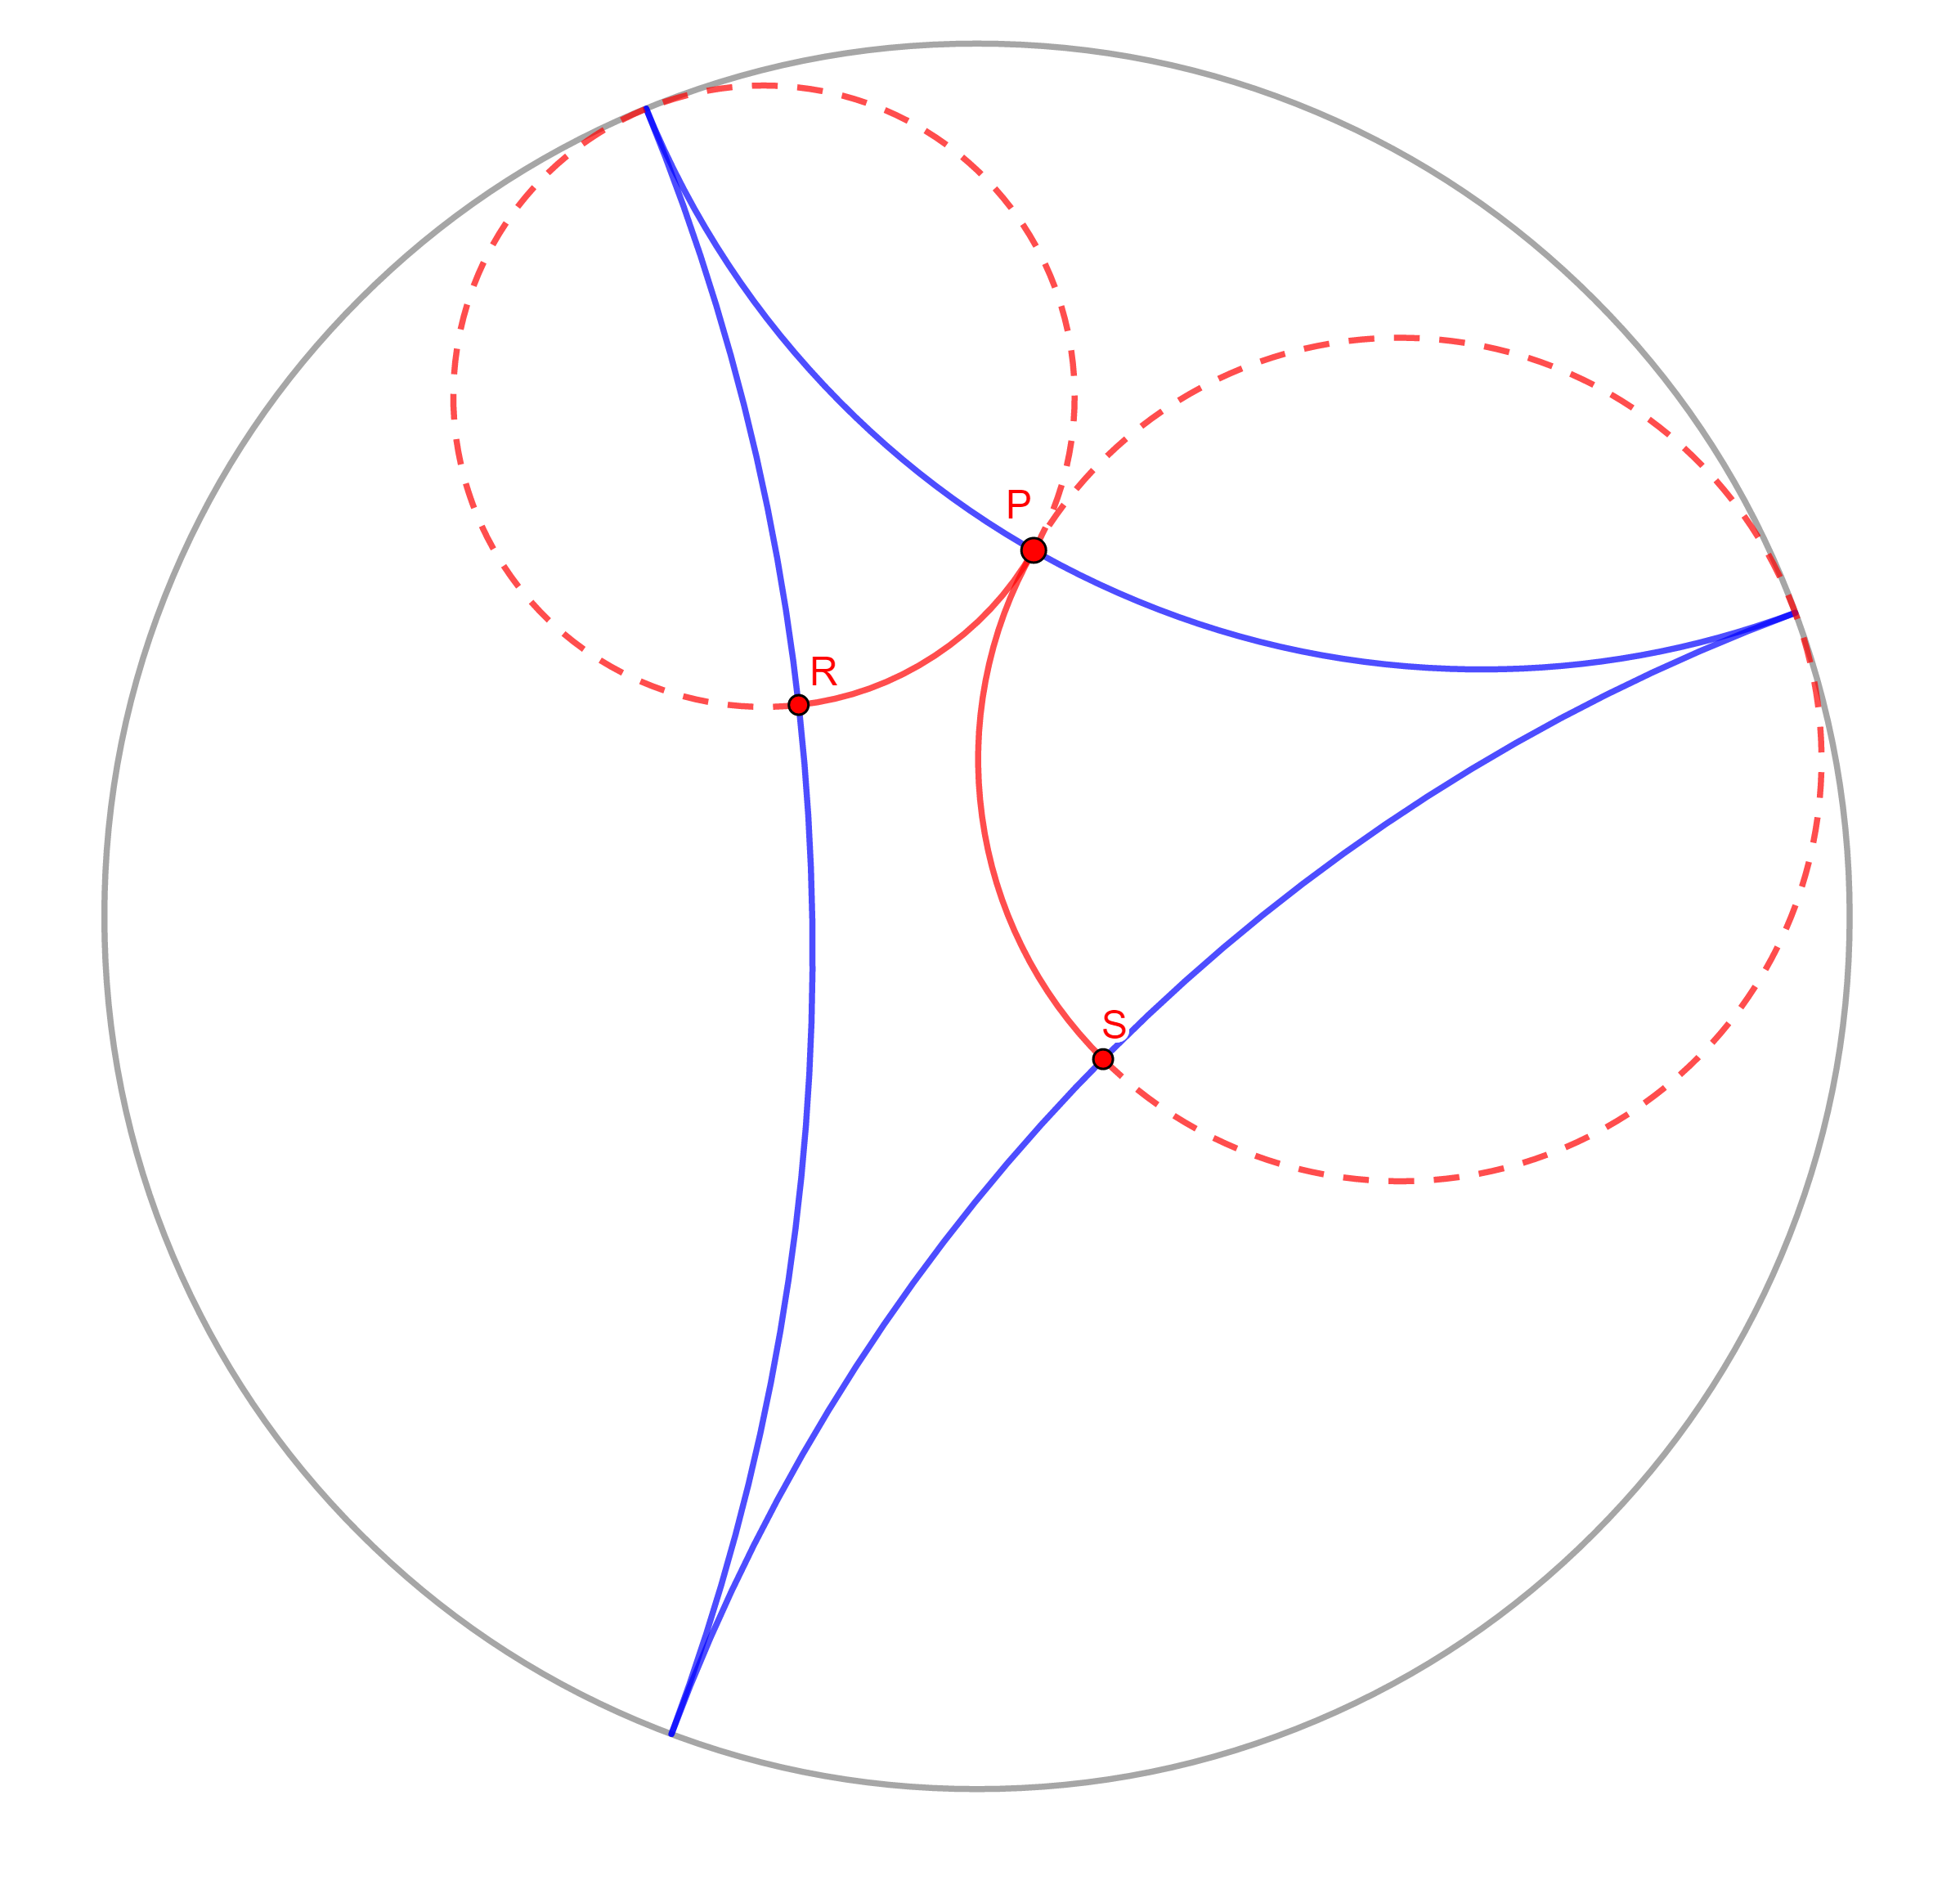
\includegraphics[width=0.5\linewidth]{pic11}
	\end{figure}
	Центр эллипсоида -- $I$, $T_1, T_2$ -- сопряженные точки
	Очевидно что $UI = QV$ и $UQ = IV$.\\
	Тогда
	\begin{gather*}
		IP^{2} = IV \cdot IT_2\\
		ID^{2} = IU \cdot IT_1 = QV \cdot IT_1\\
		\frac{IQ_1^2}{IP_1^2} = \frac{QV \cdot IT_1}{IV \cdot IT_2} = \frac{QV \cdot QV}{IV \cdot VT_2}
	\end{gather*}
	Теперь заметим что $\triangle IT_1T_2 \sim \triangle VQT_2 \sim \triangle UT_1Q$, следовательно $\frac{IT_1}{IT_2} = \frac{QV}{VT_2}$
	\begin{gather*}
		IP^2 = IV \cdot VT_2 = IV \cdot (IT_2 - IV) = IV \cdot IT_2 - IV^{2} = (IP_1 - IV)(IP_1 + IV) = VP_1 \cdot VP_2
	\end{gather*}
	Откуда
	\begin{gather*}
		\frac{IQ_1^2}{IP_1^2} = \frac{QV^2}{VP_1 \cdot VP_2}
	\end{gather*}
	Что и требовалось
\item[(б*)] 
\end{enumerate}
	